% Original book diagram: fig:mc_pi_estimation
% Book source: sections/Part_IV/monte_carlo.tex
% Original diagram authorship retained. Visual design: Ziad Mosalam.
\documentclass[11pt,border=8pt]{standalone}
\usepackage{amsmath,amssymb,graphicx,tikz}
\usetikzlibrary{arrows.meta,automata,positioning,calc,shapes.geometric,fit,backgrounds,patterns}
\newcommand{\vect}[1]{\mathbf{#1}}
\newcommand{\mat}[1]{\mathbf{#1}}
\newcommand{\Normal}{\mathcal{N}}
\newcommand{\prob}{p}
\newcommand{\E}{\mathbb{E}}
\newcommand{\Var}{\mathrm{Var}}
\newcommand{\Cov}{\mathrm{Cov}}
\newcommand{\CovP}{\mathbf{P}}
\newcommand{\Prob}{\mathbb{P}}
\setlength{\textwidth}{6.5in}
% Shared visual vocabulary for the book's original diagrams.
% Figures opt in explicitly, so unrelated text and existing additions are unchanged.
\definecolor{BookBlue}{HTML}{003262}
\definecolor{BookGold}{HTML}{B17A00}
\definecolor{BookTeal}{HTML}{247C86}
\definecolor{BookInk}{HTML}{30363B}
\definecolor{BookLight}{HTML}{E9EFF5}
\tikzset{
  book figure/.style={font=\small\rmfamily, color=BookBlue, text=BookInk,
    line width=0.8pt, >=Latex},
  book axis/.style={->, draw=BookInk, line width=0.6pt},
  book link/.style={->, draw=BookBlue, line width=0.8pt},
  book observation/.style={draw=BookGold, fill=BookGold!8},
  book state/.style={draw=BookBlue, fill=BookLight},
  book note/.style={font=\footnotesize\rmfamily, text=BookInk}
}

\begin{document}
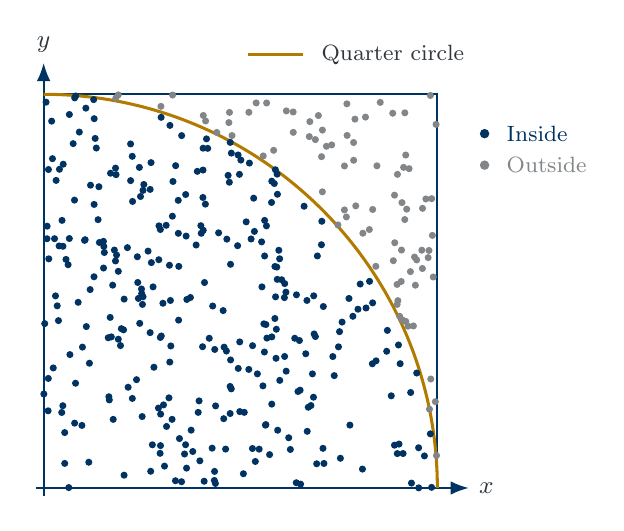
\begin{tikzpicture}[font=\small, text=BookInk, draw=BookBlue, line width=0.8pt, >=Latex, scale=5]

% Square boundary
\draw[line width=0.8pt] (0,0) rectangle (1,1);

% Axes
\draw[->] (-0.02,0) -- (1.08,0) node[right] {$x$};
\draw[->] (0,-0.02) -- (0,1.08) node[above] {$y$};

% Quarter circle
\draw[line width=1.1pt, BookGold] (1,0) arc[start angle=0,end angle=90,radius=1];

% Red legend marker + label
\draw[line width=1.1pt, BookGold] (0.52,1.10) -- (0.66,1.10);
\node[anchor=west] at (0.68,1.10) {\footnotesize Quarter circle};

% 400 pseudo-random points, uniform in the unit square (fixed seed for reproducibility)
\pgfmathsetseed{2026}
\foreach \i in {1,...,400} {
\pgfmathsetmacro{\px}{rnd}
\pgfmathsetmacro{\py}{rnd}
\pgfmathtruncatemacro{\inside}{(\px*\px+\py*\py<1) ? 1 : 0}
\ifnum\inside=1
\fill[BookBlue] (\px,\py) circle (0.009);
\else
\fill[BookInk!60] (\px,\py) circle (0.009);
\fi
}

% Legend (outside the square)
\fill[BookBlue] (1.12,0.90) circle (0.012);
\node[BookBlue, anchor=west] at (1.15,0.90) {\footnotesize Inside};
\fill[BookInk!60] (1.12,0.82) circle (0.012);
\node[BookInk!60, anchor=west] at (1.15,0.82) {\footnotesize Outside};

\end{tikzpicture}
\end{document}
